This solution is designed for cyclobutadiene anion instead of just cyclobutadiene which is the prototypical antiaromatic hydrocarbon with 4 $\pi$ electrons. Its rectangular structure is the result of a pseudo-(or second order) Jahn–Teller effect, which distorts the molecule and lowers its symmetry, converting the triplet to a singlet ground state. This distortion indicates that the $\pi$ electrons are localized, in agreement with H{\"u}ckel's rule which predicts that a $\pi$-system of 4 electrons is not aromatic. This information is excerpted from \url{https://en.wikipedia.org/wiki/Cyclobutadiene}.
		
		Firstly, it is easy find that cyclobutadiene anion belongs to the point group $\mathscr{D}_{\rm 4h}$. However, it has only 4 $\pi$-electrons. Just $\mathscr{D}_{\rm 4}$ is good enough and its character table is shown in \Tableref{tab:chatab_3}.
		\begin{center}
		\setlength{\abovecaptionskip}{0em}
		\captionof{table}{The character table for the $\mathscr{D}_{\rm 4}$ point group.}\label{tab:chatab_3}
		\begin{tabular}{cccccc}\hline
	$\mathscr{D}_{\rm 4}$ & $E$ & $2C_4$ &	$C_2$	& $2C^\prime_2$ & $2C^{\prime\prime}_2$ \\ \hline
			$A_1$	&	1	&	1	&	1	&	1	&	1	\\
			$A_1$	&	1	&	1	&	1	&	-1	&	-1	\\
			$B_1$	&	1	&	-1	&	1	&	1	&	-1	\\
			$B_2$	&	1	&	-1	&	1	&	-1	&	1	\\
			$E$ 	&	2	&	0	&	-2	&	0	&	0\\ \hline
		\end{tabular}
		\end{center}
		
		Secondly, we mark all carbon atoms as follows.
		\begin{center}
		\setlength{\abovecaptionskip}{-0.5em}
		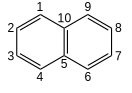
\includegraphics[scale=1.0]{./structures/exercise_1/cyclobutadiene_anion/0.png}
		\captionof{figure}{The order of carbon atoms in the cyclobutadiene anion.}\label{fig:case3}
		\end{center}
		
		For $\pi$-electron atomic orbitals' representation $\Gamma^{\rm AO}$, its following characters is listed below.
		\begin{center}
		\setlength{\abovecaptionskip}{-0.3em}
		\captionof{table}{The character of the $\pi$-electron atomic orbitals' representation $\Gamma^{\rm AO}$.}
		\begin{tabular}{cccccc}\hline
	$\mathscr{D}_{\rm 4}$	& $E$ & $2C_4$ &	$C_2$	& $2C^\prime_2$ & $2C^{\prime\prime}_2$ \\ \hline
	$\chi^{\AO}(C_i)$	&	4	&	0	&	0	&	0	&	-2	\\ \hline
		\end{tabular}
		\end{center}
		
		Relevant reduction coefficients are
		\begin{equation*}
		a_1 = 0, \quad a_2 = 1, \quad b_1 = 1, \quad b_2 = 0, \quad e = 1.
		\end{equation*}
		Then, we arrive at		
		\begin{equation*}
			\Gamma^{\AO} = \Gamma^{A_2} \oplus \Gamma^{B_1} \oplus \Gamma^{E}.
		\end{equation*}
		Thus, to describe the effect of $O_R$, two suitable $2\orbp_{z}$ atomic orbitals is enough. 
		
		Thirdly, we inspect the transformation of $\phi_i$ under $O_R$ for the cyclobutadiene anion, whose information is recorded below. We only list two $\phi_1$ and $\phi_2$.
		\begin{center}
		\setlength{\abovecaptionskip}{-0.5em}
		\captionof{table}{Transformation of $\phi_i$ under $O_R$ for the cyclobutadiene anion.}
		\begin{tabular}{ccccccccc}\hline
	$\mathscr{D}_{\rm 4}$ & $E$ & $C_4$ & $C_2$ & $C^3_4$	&	$C^\prime_{2,1}$	&	$C^\prime_{2,2}$ &	$C^{\prime\prime}_{2,1}$	&	$C^{\prime\prime}_{2,2}$	\\ \hline
			$\phi_1$	&	$\phi_1$	&	$\phi_2$	&	$\phi_3$	&	$\phi_4$	&	$-\phi_2$	&	$-\phi_4$	&	$-\phi_3$	&	$-\phi_1$	\\
			$\phi_2$	&	$\phi_2$	&	$\phi_3$	&	$\phi_4$	&	$\phi_1$	&	$-\phi_1$	&	$-\phi_3$	&	$-\phi_2$	&	$-\phi_4$	\\ \hline
		\end{tabular}
		\end{center}
		
		For the irreducible representation $\Gamma^{A_2}$, the only basis function is
		\begin{align*}
			P^{A_2}\phi_1 &= \sum_{R} \chi^{A_2}(R) O_R \phi_1 = (O_E + O_{C_4} + O_{C_2} + O_{C^3_4} - \sum_{k=1}^2 O_{C^\prime_{2,k}} -\sum_{k=1}^2 O_{C^{\prime\prime}_{2,k}} )\phi_1 \\
			&= 2(\phi_1+\phi_2+\phi_3+\phi_4).
		\end{align*}
		It can be normalized to
		\begin{equation}
			\Phi^\pi_1 = \frac{1}{2}(\phi_1+\phi_2+\phi_3+\phi_4).
		\end{equation}
		
		Then, the effective Hamiltonian for $\pi$ electrons is
		\begin{equation*}
			H^\prime = ( \alpha + 2\beta ).		
		\end{equation*}
		
		In another words, its only eigenvalue is $\alpha + 2\beta$, with eigenfunction $\Phi^\pi_1$.
		
		In conclusion, for the irreducible representation $\Gamma^{A_2}$, relevant results are listed below.
		
		\begin{center}
		\setlength{\abovecaptionskip}{0em}
		\captionof{table}{The H{\"u}ckel MOs in the irreducible representation $\Gamma^{A_2}$ of cyclobutadiene anion.}
		\begin{tabular}{ccc}\hline
		  order	&	eigenvalue		& 	eigenfunction	\\ \hline
			1	&$\alpha+2\beta$& 	$0.5000\phi_1 + 0.5000 \phi_2 + 0.5000 \phi_3 + 0.5000 \phi_4$ \\ \hline
		\end{tabular}
		\end{center}
		
		For the irreducible representation $\Gamma^{B_1}$, the only basis function is
		\begin{align*}
			P^{B_1}\phi_1 &= \sum_{R} \chi^{B_1}(R) O_R \phi_1 = 2(\phi_1 - \phi_2 + \phi_3 - \phi_4).
		\end{align*}
		It can be normalized to
		\begin{equation}
			\Phi^\pi_2 = \frac{1}{2}(\phi_1 - \phi_2 + \phi_3 -\phi_4).
		\end{equation}
		
		Then, the effective Hamiltonian for $\pi$ electrons is
		\begin{equation*}
			H^\prime = ( \alpha - 2\beta ).		
		\end{equation*}
		
		In another words, its only eigenvalue is $\alpha - 2\beta$, with eigenfunction $\Phi^\pi_2$.
		
		In conclusion, for the irreducible representation $\Gamma^{B_1}$, relevant results are listed below.
		
		\begin{center}
		\setlength{\abovecaptionskip}{0em}
		\captionof{table}{The H{\"u}ckel MOs in the irreducible representation $\Gamma^{B_1}$ of cyclobutadiene anion.}
		\begin{tabular}{ccc}\hline
		  order	&	eigenvalue		& 	eigenfunction	\\ \hline
			1	&$\alpha-2\beta$& 	$0.5000\phi_1 - 0.5000 \phi_2 + 0.5000 \phi_3 - 0.5000 \phi_4$ \\ \hline
		\end{tabular}
		\end{center}
		
		For the irreducible representation $\Gamma^{E}$, the only two basis functions are
		\begin{align*}
			P^{E}\phi_1 &= \sum_{R} \chi^{E}(R) O_R \phi_1 = 2(\phi_1 - \phi_3 ), \\
			P^{E}\phi_2 &= \sum_{R} \chi^{E}(R) O_R \phi_2 = 2(\phi_2 - \phi_4 ).	
		\end{align*}
		They can be normalized to
		\begin{align*}
			\phi^\prime_3 &= \frac{1}{\sqrt{2}}(\phi_1 - \phi_3), \\
			\phi^\prime_4 &= \frac{1}{\sqrt{2}}(\phi_2 - \phi_4).
		\end{align*}
		
		Then, the effective Hamiltonian for $\pi$ electrons is
		\begin{equation*}
			H^\prime = \begin{pmatrix}
				\alpha	&	0	\\
				0	&	\alpha
				\end{pmatrix}.				
		\end{equation*}
		It has a two-fold eigenvalue $\alpha$. Thus, corresponding eigenfunctions can be
		\begin{align}
			\Phi^\pi_3 &= \frac{1}{\sqrt{2}}(\phi_1 - \phi_3), \\
			\Phi^\pi_4 &= \frac{1}{\sqrt{2}}(\phi_2 - \phi_4).
		\end{align}
		
		In another words, its only eigenvalue is $\alpha$, with two eigenfunctions $\Phi^\pi_3$ and $\Phi^\pi_4$.
		
		In conclusion, for the irreducible representation $\Gamma^{E}$, relevant results are listed below.
		
		\begin{center}
		\setlength{\abovecaptionskip}{0em}
		\captionof{table}{The H{\"u}ckel MOs in the irreducible representation $\Gamma^{E}$ of cyclobutadiene anion.}
		\begin{tabular}{ccc}\hline
		  order	&	eigenvalue		& 	eigenfunction	\\ \hline
			1	&$\alpha$& 	$0.7071\phi_1 - 0.7071 \phi_3$ \\ 
			2	&$\alpha$& 	$0.7071\phi_2 - 0.7071 \phi_4$ \\\hline
		\end{tabular}
		\end{center}
		
		Now, we have obtained all results, which are shown as following.
		
		\begin{center}
		\setlength{\abovecaptionskip}{-0.5em}
		\captionof{table}{The H{\"u}ckel MOs in all irreducible representations of cyclobutadiene anion.}
		\begin{tabular}{ccccccc}\hline
		order 	& orbital energy & irrep & $c_1$ & $c_2$ & $c_3$ &$c_4$ \\ \hline
			1	&	$\alpha+2.000\beta$	&	$A_2$	&	0.5000	&	0.5000	&	0.5000	&	0.5000	\\
			2	&	$\alpha$	&	$E$	&	0.7071	&	0.0000	&	-0.7071	&	0.0000	\\
			3	&	$\alpha$	&	$E$	&	0.0000	&	0.7071	&	0.0000	&	-0.7071	\\
			4	&	$\alpha-2.000\beta$	&	$B_1$	&	0.5000	&	-0.5000	&	0.5000	&	-0.5000	\\ \hline
		\end{tabular}
		\end{center}
		
		Besides, their phase diagrams have been painted in \Figref{fig:phase_diagram_3}.
		
		\begin{center}
		\begin{tabular}{cccc}
			\begin{minipage}[t]{0.22\linewidth}
			\centering
			\setlength{\abovecaptionskip}{0.5em}
			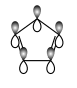
\includegraphics[scale=1]{./structures/exercise_1/cyclobutadiene_anion/1.png}
			\captionof*{figure}{$\varepsilon = \alpha + 2.000\beta$}
			\end{minipage} & 
			\begin{minipage}[t]{0.22\linewidth}
			\setlength{\abovecaptionskip}{0.5em}\hspace*{2em}
			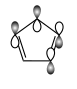
\includegraphics[scale=1]{./structures/exercise_1/cyclobutadiene_anion/3.png}
			\captionof*{figure}{$\varepsilon = \alpha + 0.000\beta$}
			\end{minipage} &
			\begin{minipage}[t]{0.22\linewidth}
			\centering
			\setlength{\abovecaptionskip}{0.5em}
			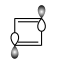
\includegraphics[scale=1]{./structures/exercise_1/cyclobutadiene_anion/4.png}
			\captionof*{figure}{$\varepsilon = \alpha + 0.000\beta$}
			\end{minipage} & 
			\begin{minipage}[t]{0.22\linewidth}
			\setlength{\abovecaptionskip}{0.5em}\hspace{2em}
			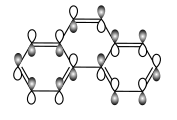
\includegraphics[scale=1]{./structures/exercise_1/cyclobutadiene_anion/2.png}
			\captionof*{figure}{$\varepsilon = \alpha - 2.000\beta$}
			\end{minipage}
		\end{tabular}				
		\captionof{figure}{Phase diagrams of these H{\"u}ckel MOs of cyclobutadiene anion. Black bubbles mean plus phase while white ones mean minus phase. The color is used just for determining relative phase.}\label{fig:phase_diagram_3}
		\end{center}
		
		In the end, we conclude that for cyclobutadiene anion, its ground state $\pi$-electron configuration is $(a_2)^2(e)^4$ and its delocalization energy is $-2.000\beta$, which means that cyclobutadiene anion needs other stable structures to stabilize itself.